
\section{Similar Solutions}

\subsection{Sentiment Analysis Products}
There are many existing sentiment analysis projects that use machine learning to predict how positive or negative (the valence) of input text.

The Amazon Web Services (AWS) Platform offers Amazon Comprehend \cite{aws} which is an example of this. 

Amazon Comprehend is a NLP tool that extracts the following from input text:
\begin{center}
\begin{tabular}{ |c|c| } 
 \hline
  Categories & Examples \\ 
 \hline                        
 Entities & People, Places, Locations\\
 Key Phrases & The most important parts of the input text \\
 Language & English \\
 Sentiment & Positive, Negative or Mixed \\
 Syntax & Verbs, Pronouns, Proper Nouns \\
 \hline
\end{tabular}
\end{center}

Since only the sentiment is interesting to us here,and the insight the tool provides is limited as it only measures valence, and when tested with a confusing piece text it performed badly, as shown in Figure \ref{aws:sentiment}. This is a clear example of a tool which can be improved upon

\begin{figure}[ht]
\caption{Image showing the input text and incorrect analysis of the sentiment of it by the Amazon Comprehend service}
\centering
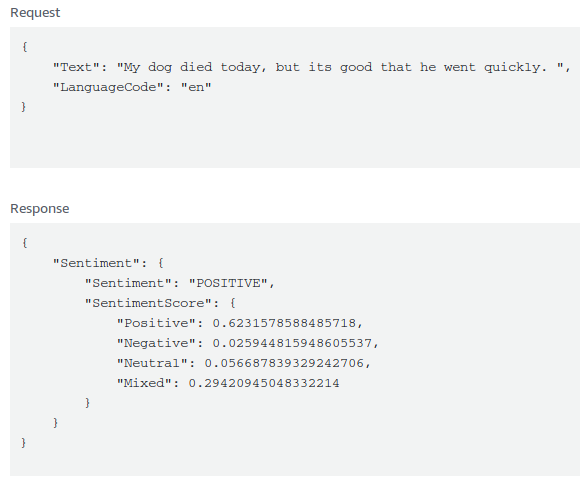
\includegraphics[scale=0.5]{./LitReview/images/comphrendResult.png}
\label{aws:sentiment}
\end{figure}

Getting confused with sentences that are actually negative, but include words like 'happy' is common issue with existing sentiment tools and one that should be solved by not only analysing the valence of a text, but looking at the text in more ways than just the positivity of it and taking into account the whole sentence.

\subsection{Sentiment Analysis Research}

There seems to be very little existing work which tries to use semantic analysis to predict more than just the valence of text, as most existing work is only considering how positive or negative the input is. Attempting to predict a more descriptive form of the emotion of the input will be a challenge.

When analysing the positivity and negativity of tweets, using a lexicon based approach as well as machine learning approaches have been used \cite{kolchyna2015twitter} \cite{go2009twitter} to great effect. In this case, a combination of the two has proved to be the most effective. Investigating whether these approaches work just as well when taking into account more than just the valence of the text will be the majority of the work on this project.

Existing sentiment analysis research processes the data a large amount before any machine learning is done on it, for example by removing all the words which lie exactly in the middle of the valence scale.  \cite{kolchyna2015twitter} The different pre-processing methods will also be compared during this project.

\subsection{Spotify}
With Spotify API being very easy to access for developers, there already exists large numbers of web applications that utilise the data that Spotify provides. Creating a basic web app with HTML front and a Node.js back end is very straightforward \cite{spotifyHello}, with extensive documentation being provided by Spotify, and there are many other online sources to facilitate the building of this part of the application. 

A project which is similar to the Spotify API that will be created as part of the web application that will showcase the output of the sentiment analysis tool is the MoodTape web app, which generates playlists using the users top artists and a valence value between 0 and 1 \cite{moodtape}.
In the production of this application, it was discovered that some songs which would be described as 'popular party songs' are valued with low valence scores due to having a large amount of minor chords. To deal with this, they incorporated the energy and danceability attributes. 
This application only takes in values from 0 to 1 as a mood, and an improvement that could be made is to try and move away from inputting numeric values to inputting a mood. The use of creating the playlist based on the users top artists is something that was not considered before, and now will be factored into future production plans.

The Spotify solution to be created will be a RESTful API built with Node.js, which has already been prototyped and will be easy to continue work on, due the the amount of documentation available \cite{spotifyHello}.

\begin{lstlisting}[style=leftCode, caption={Some of the attributes of a song obtained through requesting information through the Spotify API},captionpos=b, label={spotifyJSON}]
{
    "danceability": 0.322,
    "energy": 0.0593,
    "key": 1,
    "loudness": -53.057,
    "speechiness": 0.0444,
    "acousticness": 0.908,
    "instrumentalness": 0.708,
    "liveness": 0.121,
    "valence": 0.0165,
    "tempo": 158.402,
    "time_signature": 4
}
\end{lstlisting}